\setcounter{chapter}{+1}

Ao introduzir uma linguagem de programação é comum nos ensinarem a organizar conjuntos de dados (um conjunto de números inteiros, float, double, etc;). Esses conjuntos de dados podem ser mantidos em uma estrutura de dados que conhecemos como vetores e/ou matrizes, esses vetores e matrizes são blocos de memórias sequências que são responsáveis por facilitar a manipulação e acesso a informação que desejamos manipular.\par
Quando precisamos organizar esse conjunto de dados em ordem crescente, decrescente ou seguindo algum padrão específico é comum utilizarmos algoritmos de organização como o bubble sort, por exemplo. Quando trabalhos com um conjunto de dados que cabe na memória e queremos organiza-lo denominamos Classificação Interna.\par
Os dados que não são suportados na memória e que queremos organizar chamamos de Classificação Externa. E para organizar e manipular esses dados foram criados diversos algoritmos. Veremos a seguir o método de substituição por seleção e a intercalção de n caminhos.

\section{Classificação Externa}

Os dados que queremos organizar estão salvos em um arquivo, a classificação externa que utilizamos para organizar estes dados pode utilizar esse arquivo original ou um arquivo auxiliar, e consiste de dois passos.\par
\textbf{Classificação:} São geradas partições(arquivos) de n registros ordenados. \par
\textbf{Intercalação:} É a transformação das partições criadas na classificação em uma única partição ordenada com todos os registros originais.\par
Tanto a Classificação quanto a Intercalação podem ser feitas por métodos variados métodos, aqui abordaremos a classificação utilizando seleção por substituição, e a intercalação de n caminhos.
\newpage
\subsection{Seleção por Substituição}

A seleção por substituição consiste basicamente da leitura do máximo de registros do arquivo original para memória, (1) selecionar o menor registro, gravar na partição de saída. Após gravar na partição de saída substituir o registro gravado pelo próximo registro do arquivo original, (2) selecionar o menor registro novamente, se o menor registro for menor que o último registro escrito no arquivo de saída então congelar este registro e ignorar no restante do processamento. Enquanto existirem registros não congelados executar a etapa (2) sucessivamente, caso contrário, fecha a partição de saída atual, descongela os registros congelados na memória, abrir nova partição de saída e executar a partir da primeira etapa novamente. 



\begin{figure}[h]
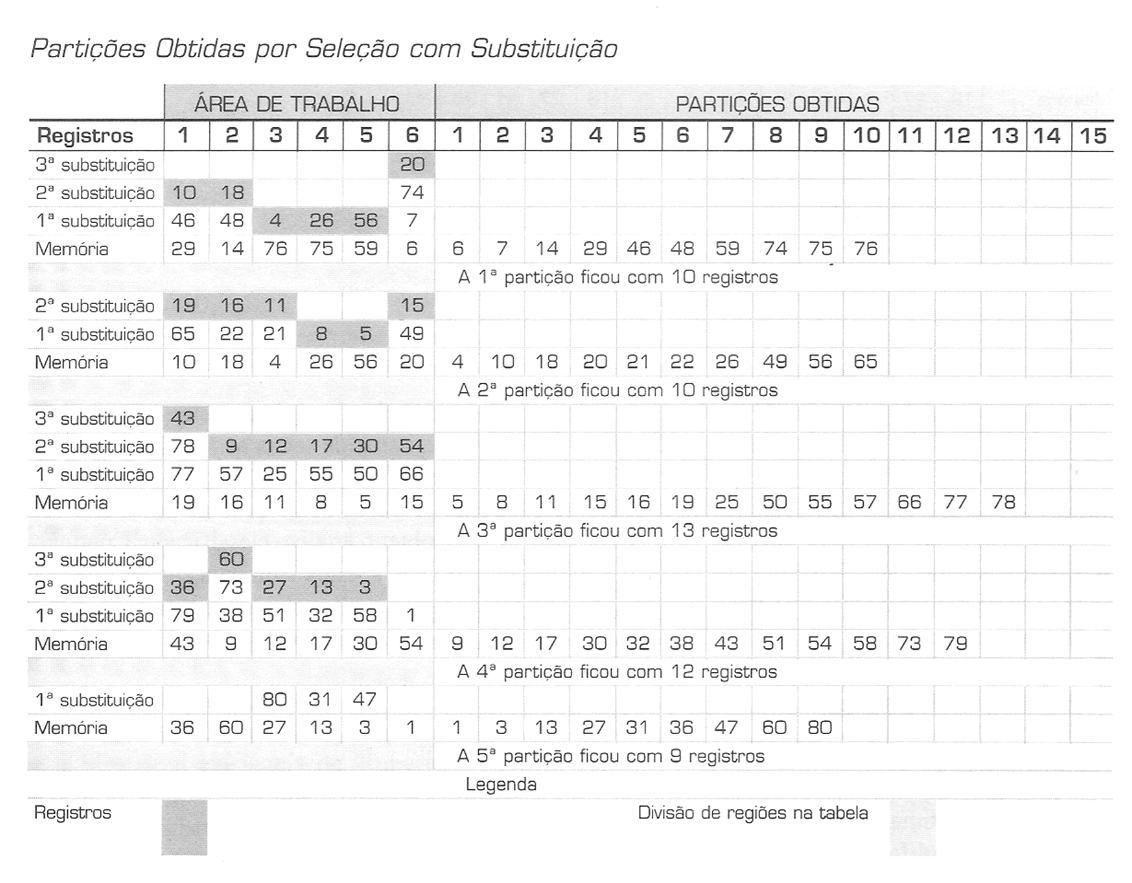
\includegraphics[width=.7\paperwidth]{selecao_com_substituicao}
\caption[align = center]{Seleção por Substituição} 
%FERRAZ, Inhaúma Neves. Programação com arquivos / Inahúma Neves Ferraz. - Barueri, SP : Manoele, 2003
\label{fig:selecao_com_substituicao}
\begin{center}
Fonte: FERRAZ, Inhaúma Neves - Programação com arquivos pg. 69
\end{center}
\end{figure}
Conforme a imagem acima, podemos observar o comportamento do método de seleção por substituição. Os registros que contém fundo escurecido são os registros que ficaram congelados e que serão utilizados no arquivo subsequente. Podemos observar que nesta etapa pode ocorrer a criação de inúmeros arquivos, e o processo só irá terminar quando não tivermos mais nenhum registro na memória e nenhum registro congelado. 
\newpage

\subsection{Balanceamento de N Caminhos}

Como vimos anteriormente a intercalação é a transformação das partições criadas na classificação em uma única partição ordenada. Para isso vamos utilizar o método de balanceamento de N caminhos.\par
Esse método consiste na união dos arquivos gerados na classificação. São N etapas unindo arquivos em duplas, ou seja, cada dois arquivos gerados na classificação um novo arquivo é gerado a partir da união. Para isso é feito a leitura registro a registro e comparando ambos. Como os arquivos estão ordenados já, então é só comparar e ir salvando um por um no novo arquivo. Ao final das N etapas teremos um arquivo final com todos os registros ordenados. Você deve estar se perguntando, mas se eu tiver um número ímpar de arquivos gerados na classificação? Isso realmente pode acontecer, para resolver isso, costumamos pegar o arquivo que sobrou na enésima etapa e unir com o primeiro arquivo gerado da etapa seguinte.

\begin{figure}[h]
\includegraphics[width=.7\paperwidth]{balanceamentoNcaminhos}
\caption{Balanceamento de N Caminhos}
\label{fig:balanceamentoNcaminhos}
\end{figure}

A ilustração acima retrata exatamente o que acontece ao intercalação, buscamos os N arquivos criados na classifição e realizamos a união em pares. Como a classificação neste caso gerou uma quantidade ímpar de arquivos, pegamos esse arquivo para utilização inicial na iteração seguinte. Isso é feito para evitar que um arquivo de tamanho muito pequeno seja mantido até o final das iterações. Neste caso garantimos que 2 arquivos de tamanhos semelhantes cheguem para ultima iteração. 
